\subsection{Radon-Nikodym and Differentiation}

% **Role:** modern integration and almost-everywhere analysis.
%
% Signed measures, absolute continuity, Radon--Nikodym theorem, Lebesgue differentiation theorem.

This subsection collects differentiation-of-measure material; signed-measure and Radon--Nikodym results can expand here later.

\begin{definition} \label{def:lebesgue-averages-and-absolute-continuity} \hlt{Averages and Absolute Continuity}\\
For $f\in\mathscr{L}^1(E)$, measurable $A\subseteq E$ with $m(A)>0$, measurable $B$, and cube or ball $Q$ with $m(Q)>0$,\\
set $[f:A]\defeq \frac{1}{m(A)}\int_A f$; and $[B:Q]\defeq \frac{m(B\cap Q)}{m(Q)}$.\\
For $f\in\mathscr{L}^1([a,b])$, an indefinite integral has form $F(x)=F(a)+\int_a^x f(t)\,dt$.\\
A function $F:[a,b]\to\R$ is \hlt{absolutely continuous} if $\forall\varepsilon>0\ \exists\delta>0\ \forall\{(a_j,b_j)\}_{j=1}^N$ finite disjoint in $[a,b]$,\\
$\sum_j(b_j-a_j)<\delta \Longrightarrow \sum_j |F(b_j)-F(a_j)|<\varepsilon$.
\end{definition}

\begin{definition} \label{def:bounded-variation-one-variable} \hlt{Bounded Variation}\\
For $F:[a,b]\to\R$, define total variation $V_a^b(F)\defeq \sup\left\{\sum\limits_{j=1}^N |F(x_j)-F(x_{j-1})|: a=x_0<x_1<\cdots<x_N=b \right\}$.\\
The function $F$ has \hlt{bounded variation} on $[a,b]$ if $V_a^b(F)<\infty$.
\end{definition}

\begin{figure}[H]
  \centering
  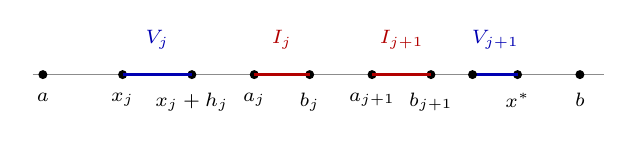
\begin{tikzpicture}[
  scale=0.88,
  every node/.style={font=\scriptsize},
  base/.style={black!45, line width=0.55pt},
  point/.style={circle, fill=black, inner sep=1.15pt},
  controlled/.style={blue!70!black, line width=1.25pt},
  gap/.style={red!70!black, line width=1.15pt},
  labelbox/.style={fill=white, inner sep=1pt}
]
  \draw[base] (-0.15,0) -- (8.1,0);

  \foreach \x/\lab in {
    0/a,
    1.15/x_j,
    2.15/{x_j+h_j},
    3.05/a_j,
    3.85/b_j,
    4.75/a_{j+1},
    5.60/b_{j+1},
    6.85/x^\ast,
    7.75/b
  } {
    \node[point] at (\x,0) {};
    \node[below=3pt] at (\x,0) {$\lab$};
  }

  \draw[controlled] (1.15,0) -- (2.15,0);
  \draw[gap] (3.05,0) -- (3.85,0);
  \draw[gap] (4.75,0) -- (5.60,0);
  \draw[controlled] (6.20,0) -- (6.85,0);
  \node[point] at (6.20,0) {};

  \node[labelbox, text=blue!70!black, above=8pt] at (1.65,0) {$V_j$};
  \node[labelbox, text=red!70!black, above=8pt] at (3.45,0) {$I_j$};
  \node[labelbox, text=red!70!black, above=8pt] at (5.18,0) {$I_{j+1}$};
  \node[labelbox, text=blue!70!black, above=8pt] at (6.53,0) {$V_{j+1}$};
\end{tikzpicture}

  \caption{Interval bookkeeping for absolute continuity.}
  \label{fig:absolute-continuity-interval-decomposition}
\end{figure}

\begin{perspective} \label{per:absolute-continuity-interval-bookkeeping} \hlt{Absolute Continuity as Interval Bookkeeping}\\
If $F(x)=\int_a^x f(t)\,dt$, by absolute continuity, disjoint intervals with small total length force small $F$ total change.\\
\end{perspective}

\begin{figure}[H]
  \centering
  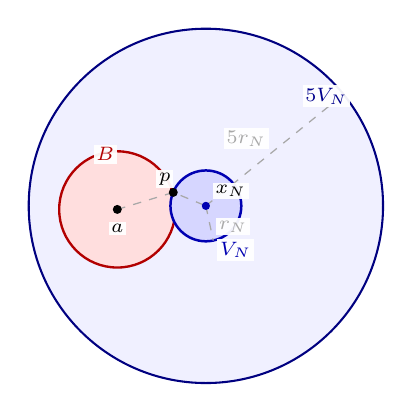
\begin{tikzpicture}[
  scale=0.90,
  every node/.style={font=\scriptsize},
  dilation/.style={draw=blue!50!black, fill=blue!6, line width=0.75pt},
  selected/.style={draw=blue!70!black, fill=blue!16, line width=0.9pt},
  missed/.style={draw=red!70!black, fill=red!13, line width=0.85pt},
  guide/.style={black!34, dashed, line width=0.45pt},
  point/.style={circle, fill=black, inner sep=1.15pt},
  center/.style={circle, fill=blue!70!black, inner sep=1.05pt},
  labelbox/.style={fill=white, fill opacity=0.94, text opacity=1, inner sep=1pt}
]
  \coordinate (x) at (0,0);
  \coordinate (a) at (-1.25,-0.05);
  \coordinate (p) at (-0.46,0.19);

  \draw[dilation] (x) circle (2.50);
  \draw[missed] (a) circle (0.82);
  \draw[selected] (x) circle (0.50);

  \draw[guide] (x) -- ++(39:2.50)
    node[pos=0.48, labelbox, above left=1pt] {$5r_N$};
  \draw[guide] (x) -- ++(-78:0.50)
    node[pos=0.60, labelbox, right=2pt] {$r_N$};
  \draw[guide] (a) -- (p) -- (x);

  \node[point] at (a) {};
  \node[center] at (x) {};
  \node[point] at (p) {};

  \node[labelbox, text=blue!70!black] at (0.42,-0.62) {$V_N$};
  \node[labelbox, text=blue!55!black] at (1.70,1.55) {$5V_N$};
  \node[labelbox, text=red!70!black] at (-1.42,0.73) {$B$};
  \node[labelbox] at (-0.58,0.38) {$p$};
  \node[labelbox] at (-1.25,-0.32) {$a$};
  \node[labelbox] at (0.35,0.21) {$x_N$};
\end{tikzpicture}

  \caption{A comparable missed ball lies inside the fivefold dilation of the selected ball.}
  \label{fig:vitali-fivefold-dilation}
\end{figure}

\begin{perspective} \label{per:vitali-covering-fivefold-control} \hlt{Vitali Covering Control}\\
In a Vitali selection, choose a pairwise disjoint subfamily by decreasing scale. If a candidate ball is not selected, it meets an earlier selected ball of comparable radius, so the fivefold dilation of that selected ball contains it.\\
\hlt{Key Insight}: Disjoint selected balls make measures add, while fixed dilations recover the missed part with bounded overlap cost.
\end{perspective}

\begin{definition} \label{def:vitali-coverings-and-density-points} \hlt{Vitali Coverings and Density Points}\\
For $A$ in a metric space $M$, $\mathcal{V}$ is a \hlt{Vitali covering} of $A$ if $\forall p\in A\ \forall r>0\ \exists V\in\mathcal{V}$ such that $p\in V$, $\diam(V)<r$.\\
For measurable $E\subseteq\R^n$, define its \hlt{density-point set} $\operatorname{dp}(E)\defeq\{p\in\R^n:\lim\limits_{Q\downarrow p}[E:Q]=1\}$, where $Q$ ranges over cubes, equivalently balls, containing $p$ and shrinking to $p$.
\end{definition}

\begin{theorem} \label{thm:vitali-covering-lemma-balls-cubes} \hlt{Vitali Covering Lemma for Balls and Cubes}\\
Let $m^\ast(E)<\infty$, and let $\mathcal{V}$ be a Vitali covering of $E\subseteq\R^n$ by closed balls or axis-parallel cubes.\\
Then there exists a countable pairwise disjoint $(V_j)\subseteq\mathcal{V}$ such that $m^\ast\left(E\setminus\bigcup\limits_{j=1}^\infty V_j\right)=0$.
\begin{proof}
Fix open $O\supseteq E$ with $m(O)<m^\ast(E)+\varepsilon$, and replace $\mathcal{V}$ by $\{V\in\mathcal{V}:V\subseteq O\}$, still a Vitali cover.\\
Choose greedily by dyadic diameter scales a maximal disjoint family $(V_j)\subseteq O$. Let $V^\ast$ be a fixed dilation such that $W\cap V\neq\varnothing,\quad \diam W\le 2\diam V$ $\Longrightarrow$ $W\subseteq V^\ast$, $m(V^\ast)\le C_n m(V)$.\\
For $R=E\setminus\bigcup_jV_j$ and each $N$, closedness gives, for every $p\in R$, a small $W\in\mathcal{V}$ with $p\in W$ and $W\cap\bigcup_{j\le N}V_j=\varnothing$. Maximality yields $W\cap V_j\neq\varnothing$ for some $j>N$ with comparable diameter, hence $R\subseteq \bigcup\limits_{j>N}V_j^\ast$.\\
Thus $m^\ast(R)\le C_n\sum\limits_{j>N}m(V_j)\to 0$, since $\sum_jm(V_j)=m(\bigsqcup_jV_j)\le m(O)<\infty$. Hence $m^\ast(R)=0$.\\
\hlt{Structural Commentary}: Vitali selection gives a disjoint cover modulo null sets.\\
\hlt{Key Insight}: $R\subseteq\bigcup_{j>N}V_j^\ast$ and disjoint tails vanish.
\end{proof}
\end{theorem}

\begin{theorem} \label{thm:lebesgue-density-theorem} \hlt{Lebesgue Density Theorem}\\
For Lebesgue measurable $E\subseteq\R^n$, $m(E\triangle\operatorname{dp}(E))=0$; and $\lim_{Q\downarrow p}[E:Q]=\mathbf{1}_E(p)$ for a.e. $p$, where $Q$ ranges over cubes, equivalently balls, shrinking to $p$.
\begin{proof}
Assume first $m(E)<\infty$. For $0<a<1$, set $E_a=\left\{p\in E:\liminf\limits_{Q\downarrow p}[E:Q]<a\right\}$.\\
The cubes $Q\ni p$ with $[E:Q]<a$ form a Vitali cover of $E_a$. Given $\varepsilon>0$, restrict to cubes in an open $O\supseteq E_a$ with $m(O)<m(E_a)+\varepsilon$, and choose disjoint $(Q_j)$ covering $E_a$ modulo null sets by Theorem \ref{thm:vitali-covering-lemma-balls-cubes}.\\
Then $m(E_a)\le \sum\limits_jm(E_a\cap Q_j) \le \sum\limits_jm(E\cap Q_j) <a\sum\limits_jm(Q_j) \le a\,m(O) <a(m(E_a)+\varepsilon)$.\\
Letting $\varepsilon\downarrow0$ gives $m(E_a)\le a\,m(E_a)$, so $m(E_a)=0$. Hence, outside $\bigcup_{a\in\Q\cap(0,1)}E_a$, points of $E$ have density $1$.\\
Apply to bounded pieces of $E^c$ to get density $0$ a.e. off $E$; apply same bounded exhaustion to remove $m(E)<\infty$.\\
\hlt{Structural Commentary}: Measurable sets are locally $0$ or $1$ a.e.\\
\hlt{Key Insight}: Vitali turns bad density into $m(E_a)\le a\,m(E_a)$.
\end{proof}
\end{theorem}

\begin{corollary} \label{cor:density-points-commute-with-slices} \hlt{Density Points Commute with Slicing Almost Everywhere}\\
Let $E\subseteq\R^n\times\R^k$ be measurable. For a.e. $x\in\R^n$, $\operatorname{dp}(E_x)=\{y:(x,y)\in\operatorname{dp}(E)\}$ up to a null subset of $\R^k$.
\begin{proof}
Set $D=\operatorname{dp}(E)$ and $N=E\triangle D$.\\
By Theorem \ref{thm:lebesgue-density-theorem}, $m_{n+k}(N)=0$; hence Theorem \ref{thm:zero-slices-null-set-criterion} gives $m_k(N_x)=0$ for a.e. $x$.\\
Intersecting with the Fubini good set, $E_x,D_x$ are measurable and $m_k(E_x\triangle D_x)=m_k((E\triangle D)_x)=0$.\\
Applying Theorem \ref{thm:lebesgue-density-theorem} in $\R^k$ gives $m_k(E_x\triangle\operatorname{dp}(E_x))=0$.\\
Therefore $m_k(\operatorname{dp}(E_x)\triangle D_x)=0$; and $m_k(\operatorname{dp}(E_x)\triangle D_x)=0$.
This is the claimed equality modulo null sets.\\
\hlt{Structural Commentary}: Almost-everywhere local fullness is compatible with almost-everywhere slicing.\\
\hlt{Key Insight}: Null ambient errors have null slices for almost every base point.
\end{proof}
\end{corollary}

\begin{lemma} \label{lem:large-average-set-bound} \hlt{Large Averages Have Small Outer Measure}\\
For a cube $Q_0\subseteq\R^n$, $g\ge0$ in $\mathscr{L}^1(Q_0)$, and $\lambda>0$,\\
set $A_\lambda\defeq \left\{p\in Q_0:\forall r>0\ \exists\text{ cube }Q\subseteq Q_0,\ p\in Q,\ \diam Q<r,\ [g:Q]>\lambda\right\}$ for $m^\ast(A_\lambda)\leq \frac{1}{\lambda}\int_{Q_0} g$.
\begin{proof}
Let $\mathcal{V}_\lambda=\{Q\subseteq Q_0:Q\text{ is a cube and }[g:Q]>\lambda\}$. By definition, $\mathcal{V}_\lambda$ is a Vitali cover of $A_\lambda$; choose disjoint $(Q_j)\subseteq\mathcal{V}_\lambda$ with $m^\ast(A_\lambda\setminus\bigcup_jQ_j)=0$. Then $\lambda m^\ast(A_\lambda) \le \lambda\sum_jm(Q_j) <\sum_j\int_{Q_j}g \le\int_{Q_0}g$.\\
\hlt{Structural Commentary}: Weak type for local averages.\\
\hlt{Key Insight}: Disjoint Vitali cubes turn pointwise large averages into one integral bound.
\end{proof}
\end{lemma}

\begin{theorem} \label{thm:lebesgue-average-value-theorem} \hlt{Lebesgue Average Value Theorem}\\
For $f\in\mathscr{L}^1_{\mathrm{loc}}(\R^n)$, $\lim\limits_{Q\downarrow p}[f:Q]=f(p)$ for a.e. $p\in\R^n$ with $Q$ cubes, equivalently balls, shrinking to $p$.
\begin{proof}
Fix a cube $Q_0$; it suffices to prove the claim for a.e. $p\in Q_0^\circ$.\\
For $\alpha>0$, let $B_\alpha=\left\{p\in Q_0^\circ:\limsup\limits_{Q\downarrow p}|[f:Q]-f(p)|>\alpha\right\}$.\\
Choose $h\in C(Q_0)$ with $\|f-h\|_{L^1(Q_0)}<\eta$, and set $g=|f-h|$. Since $[h:Q]\to h(p)$, $B_\alpha\subseteq \{g>\alpha/3\}\cup A_{\alpha/3}(g)$.\\
By Markov and Lemma \ref{lem:large-average-set-bound}, $m^\ast(B_\alpha)\le \frac{3}{\alpha}\int_{Q_0}g+\frac{3}{\alpha}\int_{Q_0}g <\frac{6\eta}{\alpha}$.\\
Let $\eta\downarrow0$; then $m(B_\alpha)=0$. Count over $\alpha\in\Q_{>0}$ and exhaust $\R^n$ by cube interiors.\\
\hlt{Structural Commentary}: Local averages recover the original integrable function almost everywhere.\\
\hlt{Key Insight}: Continuous approximation handles the good part; Vitali's estimate makes the bad part small.
\end{proof}
\end{theorem}

\begin{theorem} \label{thm:lebesgue-antiderivative-theorem} \hlt{Lebesgue's Antiderivative Theorem}\\
For $f\in\mathscr{L}^1([a,b])$, define $F(x)=c+\int_a^x f(t)\,dt$. Then $F\in AC([a,b])$ and $F'(x)=f(x)$ for a.e. $x\in[a,b]$.
\begin{proof}
Given $\varepsilon>0$, choose $\delta>0$ so that $m(A)<\delta$ implies $\int_A|f|<\varepsilon$.\\
If $(\alpha_j,\beta_j)$ are disjoint and $\sum_j(\beta_j-\alpha_j)<\delta$, then $\sum_j|F(\beta_j)-F(\alpha_j)| \le \sum_j\int_{\alpha_j}^{\beta_j}|f| =\int_{\bigcup_j(\alpha_j,\beta_j)}|f| <\varepsilon$, so $F\in AC([a,b])$. For $x,x+h\in[a,b]$, let $I_h(x)=(\min\{x,x+h\},\max\{x,x+h\})$.\\
Then $\frac{F(x+h)-F(x)}{h}=[f:I_h(x)]$. Extending $f$ by $0$ outside $[a,b]$, Theorem \ref{thm:lebesgue-average-value-theorem} in one dimension gives $[f:I_h(x)]\to f(x)$ for a.e. $x$. Hence $F'=f$ a.e.\\
\hlt{Structural Commentary}: The indefinite Lebesgue integral is the correct antiderivative for integrable functions.\\
\hlt{Key Insight}: Differentiating the integral is the same as shrinking the averaging interval.
\end{proof}
\end{theorem}

\begin{figure}[H]
  \centering
  \begin{tikzpicture}[
  scale=0.86,
  >=Stealth,
  every node/.style={font=\scriptsize},
  axis/.style={->, black!40, line width=0.5pt},
  curve/.style={blue!70!black, line width=0.9pt},
  secant/.style={orange!70!black, line width=0.7pt},
  chosen/.style={orange!85!black, line width=0.9pt},
  guide/.style={black!22, dashed, line width=0.4pt},
  tick/.style={black!50, line width=0.45pt},
  point/.style={circle, fill=black, inner sep=1.15pt},
  labelbox/.style={fill=white, fill opacity=0.94, text opacity=1, inner sep=1pt}
]
  \draw[axis] (-0.35,0) -- (7.85,0) node[right] {$x$};
  \draw[axis] (0,-0.18) -- (0,3.75) node[above] {$y$};

  \coordinate (A) at (0.85,0.62);
  \coordinate (B) at (1.55,1.17);
  \coordinate (C) at (3.20,1.40);
  \coordinate (D) at (4.30,1.86);
  \coordinate (E) at (5.28,2.54);
  \coordinate (F) at (5.98,3.15);

  \draw[curve]
    (0.35,0.43)
    .. controls (0.55,0.48) and (0.70,0.55) .. (A)
    .. controls (1.10,0.72) and (1.22,1.08) .. (B)
    .. controls (2.05,1.34) and (2.70,1.28) .. (C)
    .. controls (3.60,1.48) and (3.94,1.66) .. (D)
    .. controls (4.76,2.08) and (4.96,2.30) .. (E)
    .. controls (5.56,2.73) and (5.64,3.02) .. (F)
    .. controls (6.25,3.35) and (6.95,3.32) .. (7.45,3.40);

  \foreach \p/\q in {A/B,E/F} {
    \draw[secant] (\p) -- (\q);
    \node[point] at (\p) {};
    \node[point] at (\q) {};
  }
  \draw[chosen] (C) -- (D);
  \node[point] at (C) {};
  \node[point] at (D) {};

  \draw[guide] (C) -- (3.20,0);
  \draw[guide] (D) -- (4.30,0);
  \foreach \x in {3.20,4.30} {
    \draw[tick] (\x,0.08) -- (\x,-0.08);
  }
  \node[below=3pt] at (3.20,0) {$x$};
  \node[below=3pt] at (4.30,0) {$x+\frac1n$};

  \node[labelbox, text=blue!70!black] at (2.40,1.58) {$f$};
\end{tikzpicture}

  \caption{$g_n(x)$ is the slope of the short right secant from $x$ to $x+\frac1n$.}
  \label{fig:lebesgue-right-secants}
\end{figure}

\begin{perspective} \label{per:lebesgue-right-secants} \hlt{Right Secants and Differentiation}\\
Right quotients $g_n(x)=n\bigl(f(x+1/n)-f(x)\bigr)$ encode local slope data.\\
\hlt{Key Insight}: Secants turn differentiation into slope estimates.
\end{perspective}

\begin{theorem} \label{thm:lebesgue-last-theorem-and-consequences} \hlt{Lebesgue's Last Theorem and Consequences}\\
On $[a,b]$:
\begin{enumerate}[label=(\roman*)]
\setlength{\itemsep}{0pt}
\item $F$ monotone $\Rightarrow F'$ exists a.e.;
\item $F$ Lipschitz $\Rightarrow F'$ exists a.e.;
\item $F\in BV([a,b])\Rightarrow F'$ exists a.e.;
\item $F\in AC([a,b])\Rightarrow F\in BV([a,b])$, hence $F'$ exists a.e.
\end{enumerate}
\begin{proof}
\begin{enumerate}[label=(\roman*)]
\setlength{\itemsep}{0pt}
\item Assume $F$ nondecreasing. Let $D^+F(x)=\limsup\limits_{h\downarrow0}\frac{F(x+h)-F(x)}h$ and $D_-F(x)=\liminf\limits_{h\downarrow0}\frac{F(x+h)-F(x)}h$.\\
For $\alpha<\beta$ in $\Q$, set $A_{\alpha,\beta}=\{D_-F<\alpha<\beta<D^+F\}$. The right-secant Vitali selection of Figure \ref{fig:lebesgue-right-secants} gives $m(A_{\alpha,\beta})=0$: otherwise selected intervals with slopes $<\alpha$ and $>\beta$ contradict monotonicity of total rise. Also $m^\ast(\{D^+F>M\})\le \frac{F(b)-F(a)}{M}\to0$, so $D^+F=D_-F<\infty$ a.e.; hence $F'$ exists a.e.
\item If $F$ is $L$-Lipschitz, set $G_+(x)=F(x)+Lx$ and $G_-(x)=Lx-F(x)$. Then $G_\pm$ are nondecreasing, by (i) $\exists$ null sets $N_\pm$ s.t. $G_\pm'$ exist off $N_\pm$. For $x\notin N_+\cup N_-$, $F'(x)=\frac{G_+'(x)-G_-'(x)}{2}$, so $F'$ exists a.e.
\item If $F\in BV([a,b])$, write its Jordan decomposition $F=F(a)+V^+-V^-$ with $V^\pm$ nondecreasing. By (i), $\exists$ null sets $N_\pm$ s.t. $(V^\pm)'$ exist off $N_\pm$. For $x\notin N_+\cup N_-$, $F'(x)=(V^+)'(x)-(V^-)'(x)$, so $F'$ exists a.e.
\item If $F\in AC([a,b])$, choose $\delta$ for $\varepsilon=1$, and partition $a=x_0<\cdots<x_N=b$ with $x_i-x_{i-1}<\delta$. Grouping any refinement by these subintervals gives $V_a^b(F)\le N$, so $F\in BV([a,b])$. By (iii), $\exists Z\subset[a,b]$ with $m(Z)=0$ s.t. $F'(x)$ exists for all $x\in[a,b]\setminus Z$.
\end{enumerate}
\hlt{Structural Commentary}: Monotonicity drives all cases.\\
\hlt{Key Insight}: Vitali controls secants; decompose to monotone.
\end{proof}
\end{theorem}
